% !TEX encoding = UTF-8 Unicode
% REMEMBER TO SET LANGUAGE!
\documentclass[a4paper,10pt,norsk]{article}
\usepackage[utf8]{inputenc}
\usepackage[norsk]{babel}
% Standard stuff
\usepackage{amsmath,graphicx,varioref,verbatim,amsfonts,geometry}
% colors in text
\usepackage[usenames,dvipsnames,svgnames,table]{xcolor}
% Hyper refs
\usepackage[colorlinks]{hyperref}

% Document formatting
\setlength{\parindent}{0mm}
\setlength{\parskip}{1.5mm}

%Color scheme for listings
\usepackage{textcomp}
\definecolor{listinggray}{gray}{0.9}
\definecolor{lbcolor}{rgb}{0.9,0.9,0.9}

%Listings configuration
\usepackage{listings}
%Hvis du bruker noe annet enn python, endre det her for å få riktig highlighting.
\lstset{
	backgroundcolor=\color{lbcolor},
	tabsize=4,
	rulecolor=,
	language=python,
        basicstyle=\scriptsize,
        upquote=true,
        aboveskip={1.5\baselineskip},
        columns=fixed,
	numbers=left,
        showstringspaces=false,
        extendedchars=true,
        breaklines=true,
        prebreak = \raisebox{0ex}[0ex][0ex]{\ensuremath{\hookleftarrow}},
        frame=single,
        showtabs=false,
        showspaces=false,
        showstringspaces=false,
        identifierstyle=\ttfamily,
        keywordstyle=\color[rgb]{0,0,1},
        commentstyle=\color[rgb]{0.133,0.545,0.133},
        stringstyle=\color[rgb]{0.627,0.126,0.941}
        }
        
\newcounter{subproject}
\renewcommand{\thesubproject}{\alph{subproject}}
\newenvironment{subproj}{
\begin{description}
\item[\refstepcounter{subproject}(\thesubproject)]
}{\end{description}}

%Lettering instead of numbering in different layers
%\renewcommand{\labelenumi}{\alph{enumi}}
\renewcommand{\thesubsection}{\alph{subsection}}

%opening
\title{FYS-MEK 1110 - Oblig 3}
\author{Joakim Flatby}

\begin{document}

\maketitle
\section{}


%Oppg a
\subsection{)}

$F$: The force from the spring

$F_{R}$: Force of friction

$N$: Normal force

$G$: Gravitational force

\begin{figure}[h!]
        \centering 
        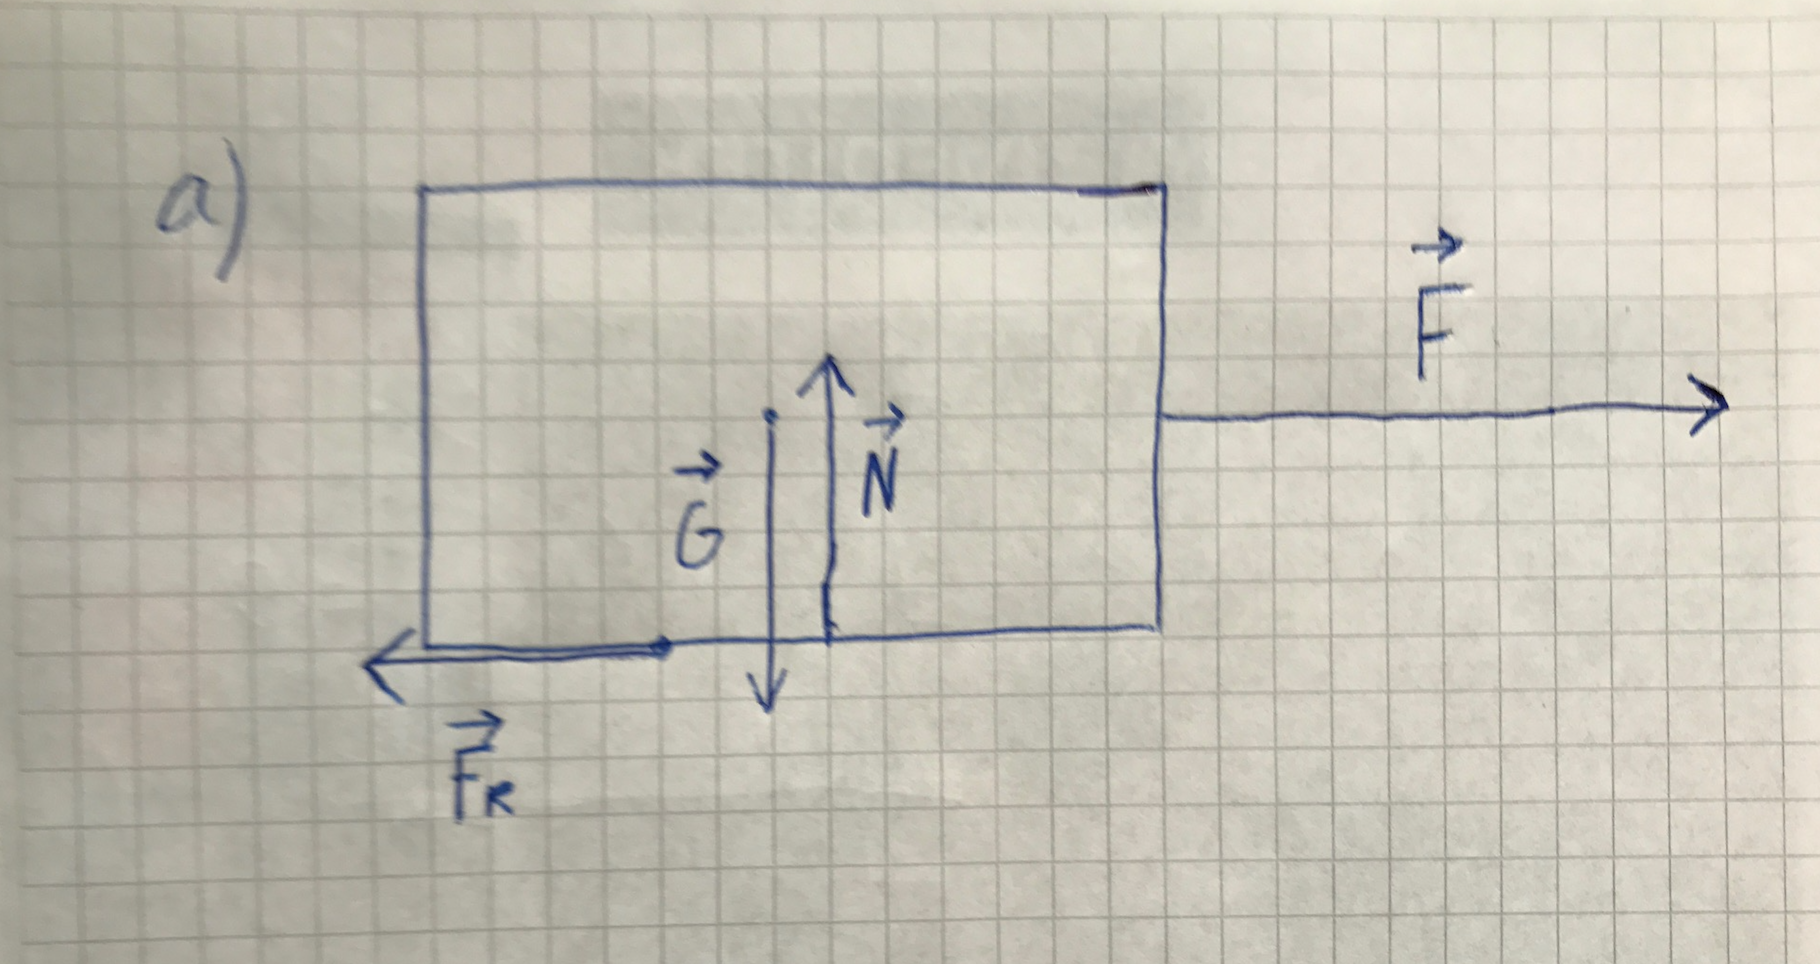
\includegraphics[scale=0.5]{oppg_a.png} 
        \caption{Flow Chart}
\end{figure}

%Oppg b
\subsection{)}
The end of the spring is moving with a constant velocity of $\vec{u}$, and we know that the initial position is $x(t0) + b$. Since $x(t0) = 0$, we get:
\[x_{b}(t) = b + \vec{u}t\]

%Oppg c
\subsection{)}
$x_{b} - x$ gives the current length of the spring. If we subtract b(equilibrium length), we get the length the spring has been stretched. So if we plug this into Hookes Law:
\[F = kx\]
\[F = k(x_{b} - x - b)\vec{i}\]
Where $\vec{i}$ is the unit vector pointing in the x-direction.

%oppg d
\subsection{)}

This is pretty much the same flow chart as in task A, except for that $F$ and $F_{R}$ are of equal length

\begin{figure}[h!]
        \centering 
        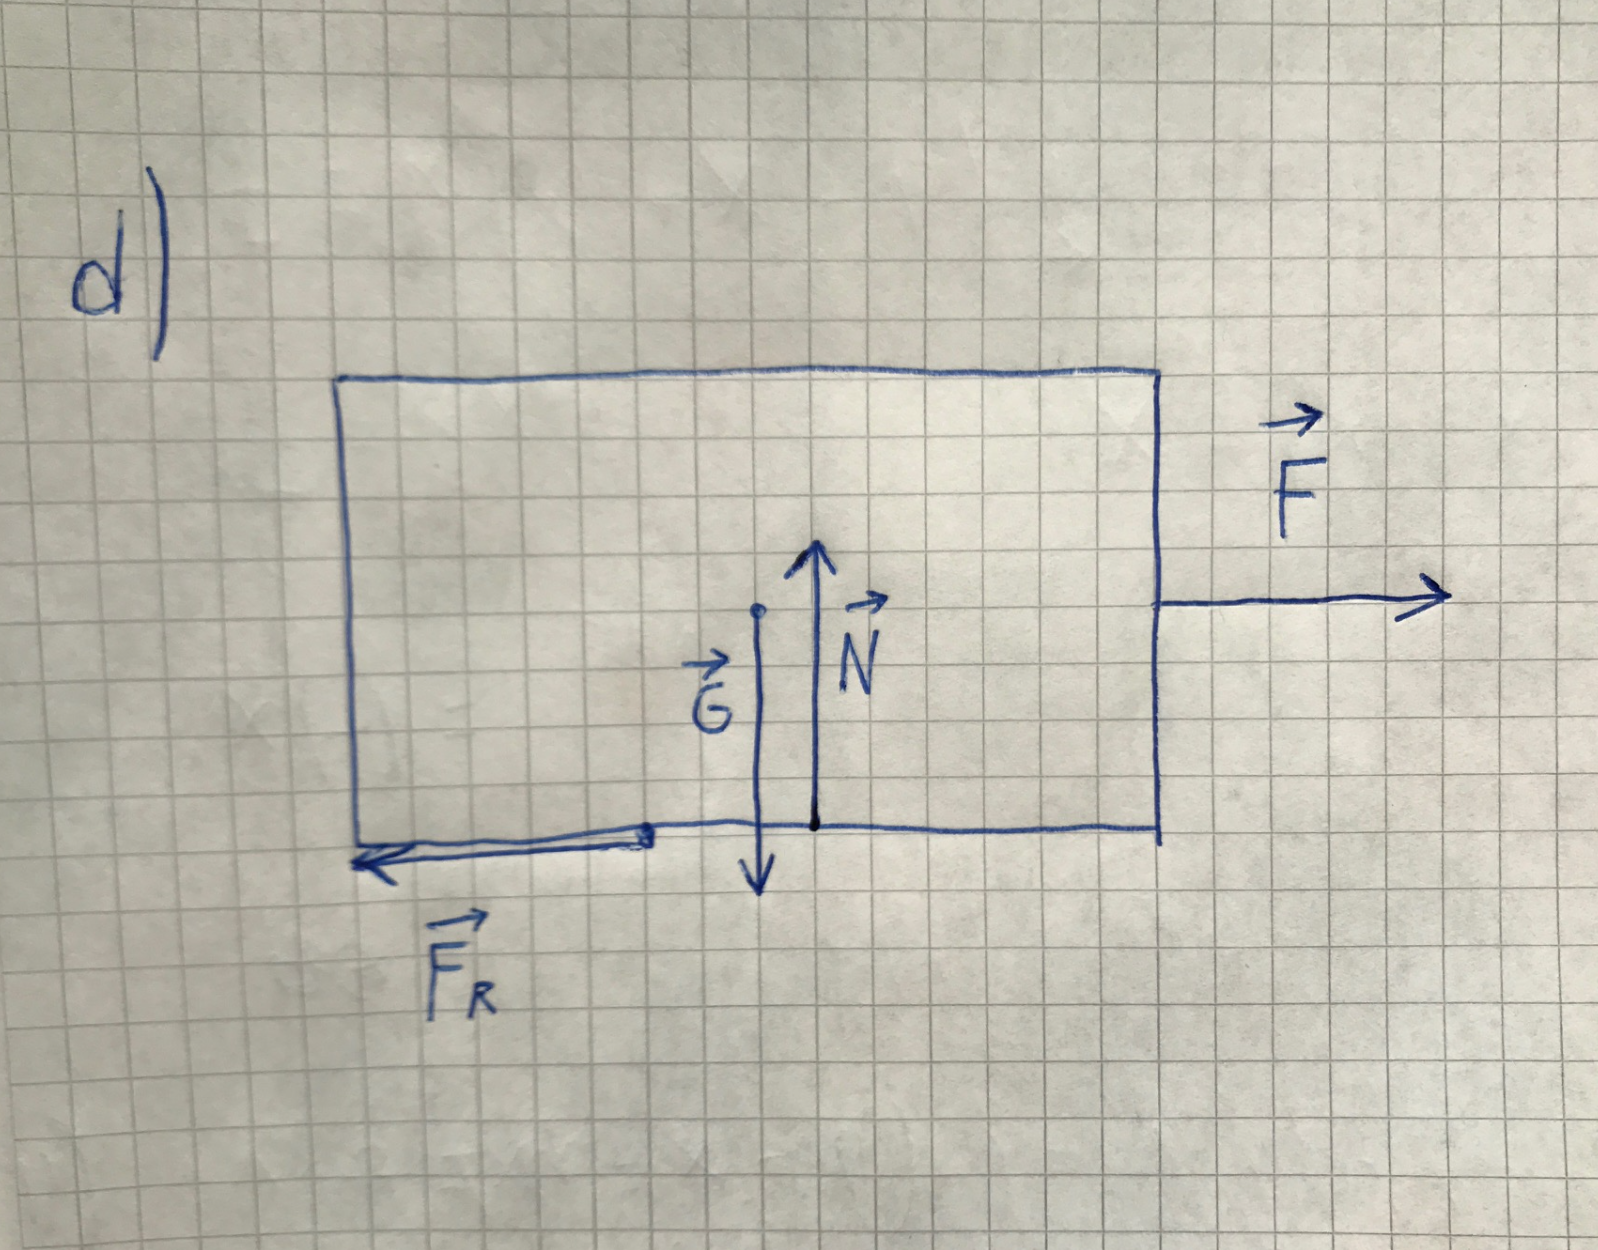
\includegraphics[scale=0.4]{oppg_d.png} 
        \caption{Flow Chart}
\end{figure}

%oppg e
\subsection{)}
Gravitational force: $\vec{G} = -mg\vec{j}$

Normal force: $\vec{N} = mg\vec{j}$

Spring force: $\vec{F} = k(x_{b} - x - b)\vec{i}$

Dynamic friction force: $\vec{F_{R}} = -\mu_{d}|\vec{N}| = -\mu_{d} mg\vec{i}$

Since the block is not moving in the y-direction, the normal force N is of equal strength and opposite direction to the gravitational force. $N = mg$

%oppg f
\subsection{)}
Seeing as the box is moving at a constant velocity in the x-direction, $a_{\vec{i}} = 0$.

And since it is not moving at all vertically(y-direction), $a_{\vec{j}} = 0$ as well.

So the acceleration of the box is 0.

%oppg g
\subsection{)}
From task C: $\Delta L = x_{b} - x - b$

So spring force can be written as: $F = k\Delta L$

We know that: $\sum F_{\vec{i}} = k\Delta L - mg\mu_{d} = 0$

Solve for $\Delta L$, and we get:
\[\Delta L = \frac{mg\mu_{d}}{k}\]


%oppg h
\subsection{)}
Since the block has a constant velocity, the position should be found by using
\[x(t) = x(t_{0}) + \vec{u}t\]
But we need to take into account the elongation of the spring, because $\vec{u}t$ only truly describes the movement of the open end of the spring.
\[x(t) = x(t_{0}) + \vec{u}t - \Delta L(t)\]
And since $x(t_{0}) = 0$, 
\[x(t) = \vec{u}t - \Delta L(t)\]

%oppg i
\subsection{)}
I copied my flow chart from task d) because this would look exactly the same.
The only difference is that the force of friction in this case is static, and not dynamic.
It is still of the same magnitude as the spring force.

Gravitational force: $\vec{G} = -mg\vec{j}$

Normal force: $\vec{N} = mg\vec{j}$

Spring force: $\vec{F} = k(x_{b} - x - b)\vec{i}$

Static friction force: $\vec{F_{R}} = -\mu_{d}|\vec{N}| = -\mu_{d} mg\vec{i}$

\begin{figure}[h!]
        \centering 
        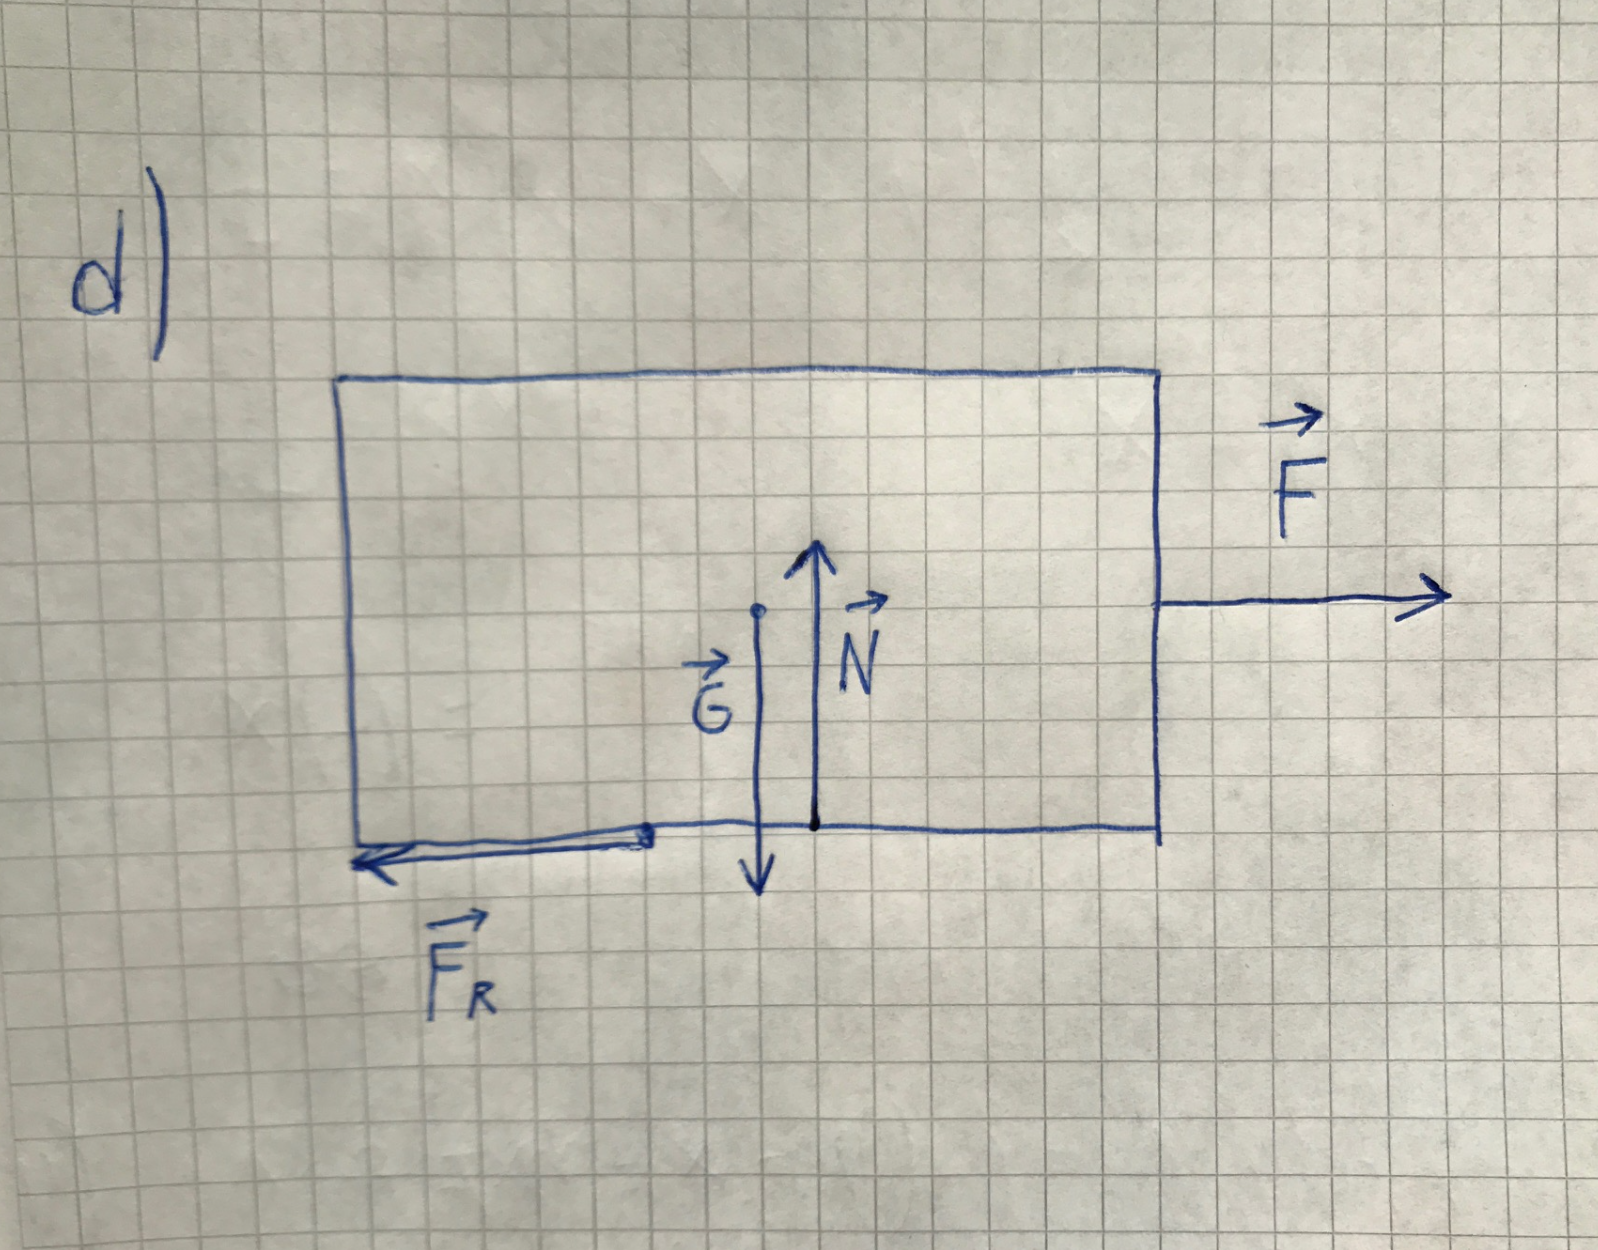
\includegraphics[scale=0.4]{oppg_d.png} 
        \caption{Flow Chart}
\end{figure}

%oppg j
\subsection{)}
Up until the block starts moving, we have:
$\sum F_{\vec{i}} = k\Delta L - mg\mu_{s} = 0$

Again, solve for $\Delta L$, and we get:
\[\Delta L = \frac{mg\mu_{s}}{k}\]


%oppg k
\subsection{)}
Since the block never moves in this scenario, the friction force will always be of equal magnitude to the spring force.

$F_{R}(t) = -F(t)$

Here we see the static friction force is increasing with F until it reaches the point where static friction cant ``hold`` the block anymore, and from there on it is the dynamic friction force, which is lower than the maximum static friction force.
\begin{figure}[h!]
        \centering 
        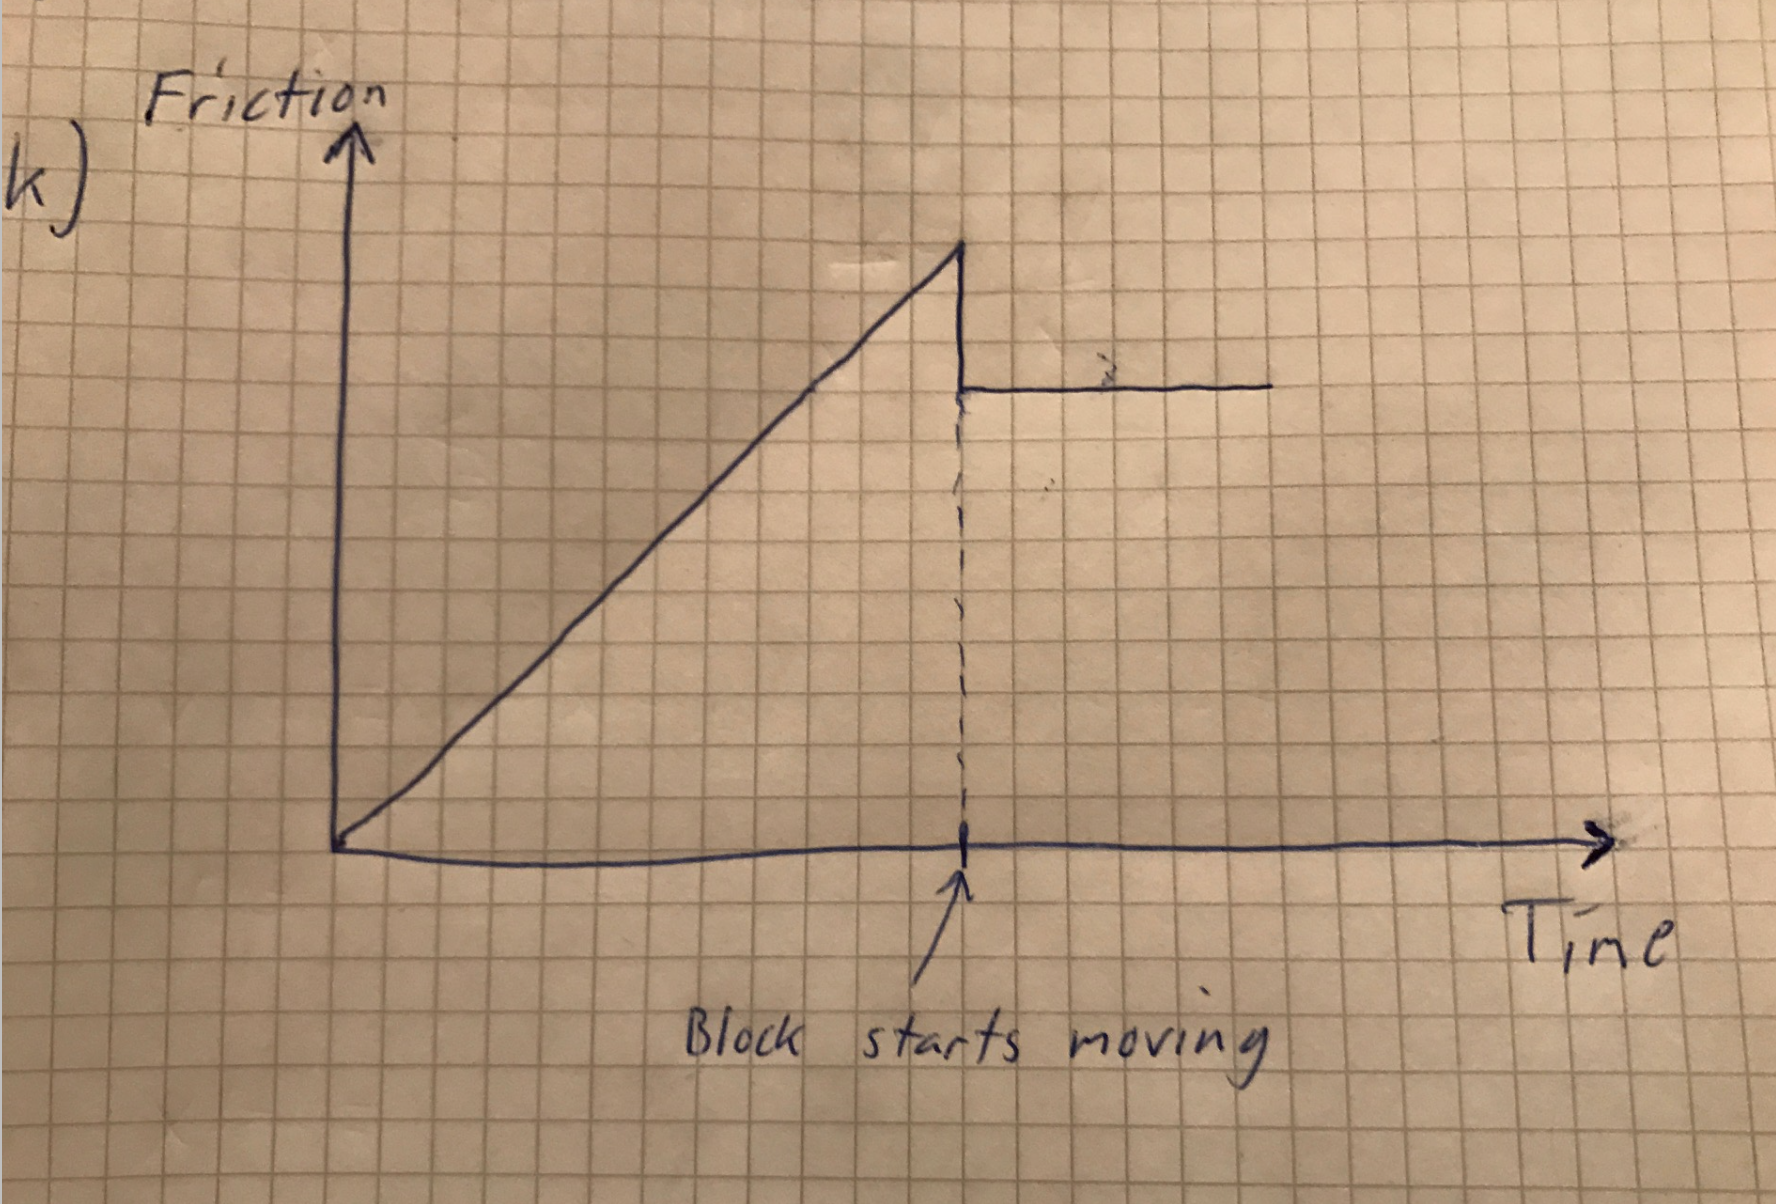
\includegraphics[scale=0.5]{oppg_k.png} 
        \caption{Flow Chart}
\end{figure}


%oppg l
\subsection{)}
\[F + F_{R} = ma\]
\[k(x_{b} - x - b) - mg\mu_{d} = ma\]
\[a = \frac{k(x_{b} - x - b) - mg\mu_{d}}{m}\]
\[a = \frac{k}{m}(x_{b} - x - b) - \mu_{d}g\]

This cannot be used to describe the entire motion of the block because it only uses the dynamic friction coefficient which isnt always the case for the block movement.

%oppg m
\subsection{)}

Gravitational force: $\vec{G} = -mg\vec{j}$

Normal force: $\vec{N} = mg\vec{j}$

Spring force: $\vec{F} = k(x_{b} - x - b)\vec{i}$

\begin{figure}[h!]
        \centering 
        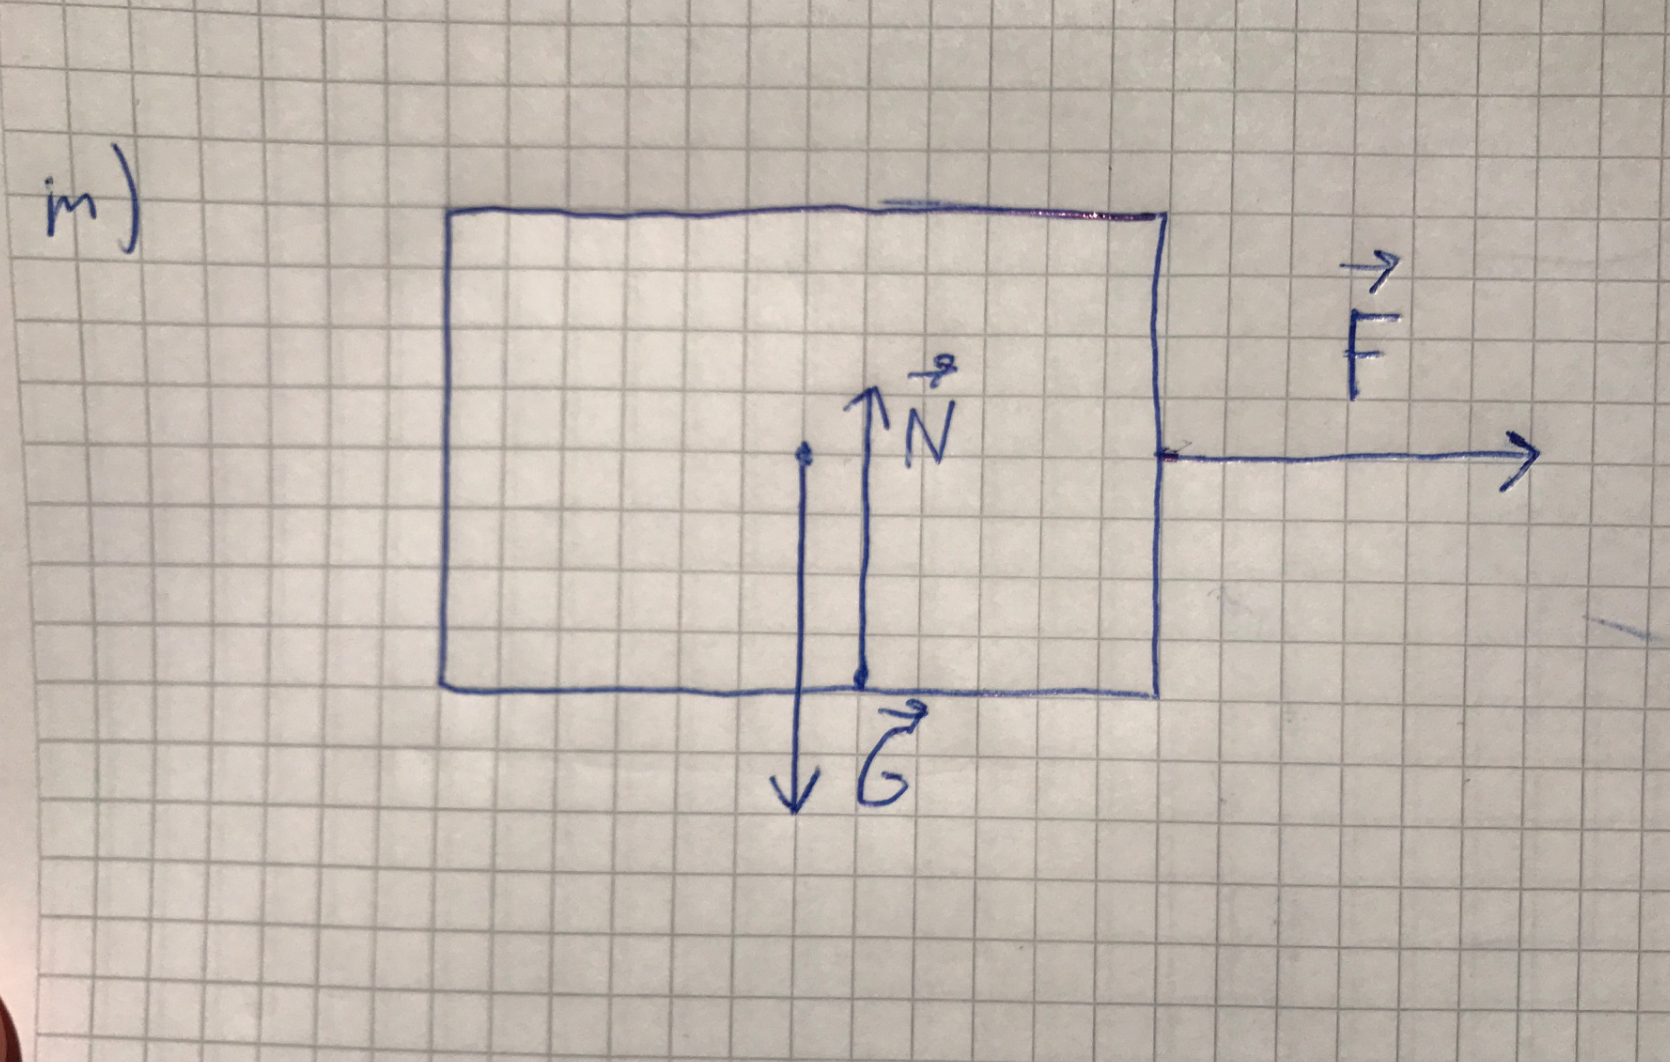
\includegraphics[scale=0.5]{oppg_m.png} 
        \caption{Flow Chart}
\end{figure}

%oppg n
\subsection{)}
The spring force is the only force acting upon the block in the x-direction, but since the spring is moving at 0m/s in this scenario, and it is already at the equilibrium length, it means that the spring force $F = 0$, which also means that the acceleration is zero.

$a_{x} = 0$

If this wasnt the case, we could find the acceleration using:

$a_{x} = \frac{k}{m}(x_{b} - x - b)$


%oppg o
\subsection{)}
Using the expression for horizontal acceleration:

$a_{x} = \frac{k}{m}(x_{b} - x - b)$

The acceleration in the x-direction is the same as the double derivative of $x(t)$:

\[x''(t) = \frac{k}{m}(x_{b} - x - b)\]
\[x''(t) = \frac{k}{m}x_{b} - \frac{k}{m}x - \frac{k}{m}b\]
Characteristic Equation:s
\[r^{2} + \frac{k}{m}r^{0} = 0\]
\[r^{2} = -\frac{k}{m}\]
\[\Downarrow\]
\[r = \pm\sqrt{-\frac{k}{m}}\]
\[r = \pm\sqrt{\frac{k}{m}}i\]

Given $\omega = \sqrt{\frac{k}{m}}$

\[r = \omega i\]
\[r = 0 + \omega i\]

Using General solution:

\[x(t) = Ce^{at}cos(\beta t) + De^{at}sin(\beta t)\]
\[x(0) = Ce^{0}cos(0) + De^{0}sin(0)\]
\[\Downarrow\]
\[C = 0\]

\[x'(0) = D\omega cos(\omega * 0) = v_{0}\]
\[\Downarrow\]
\[D = \frac{v_{0}}{\omega}\]

And with all this, we have:
\[x(t) = \frac{v_{0}}{\omega}sin(\omega t)\]

\pagebreak

%oppg p
\subsection{)}

%oppg q
\subsection{)}

\lstinputlisting{oppg_p.py}

\begin{figure}[h!]
        \centering 
        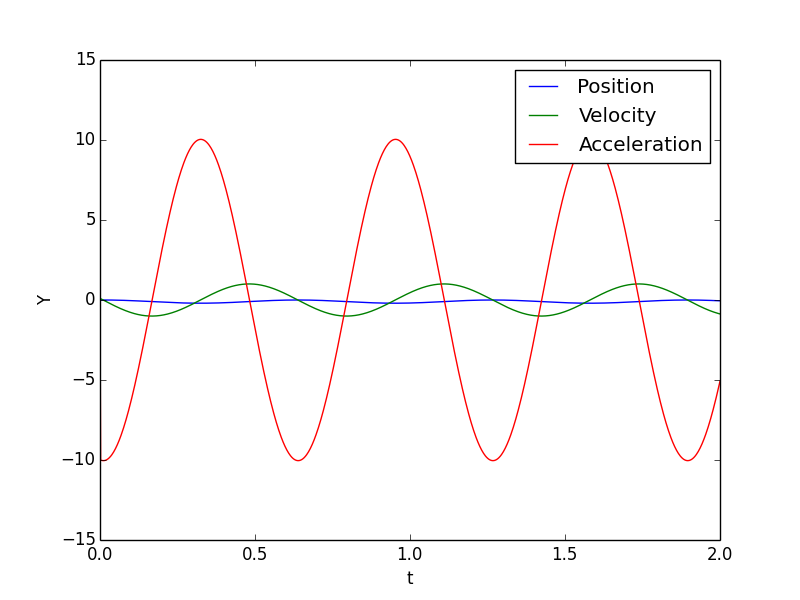
\includegraphics[scale=0.5]{oppg_p.png} 
        \caption{Graph}
\end{figure}

If we chose a too large value for $\Delta t$, the motion will not be calculated correctly because you dont ``update`` the spring force value often enough.

%oppg r
\subsection{)}
\lstinputlisting{oppg_r.py}

\begin{figure}[h!]
        \centering 
        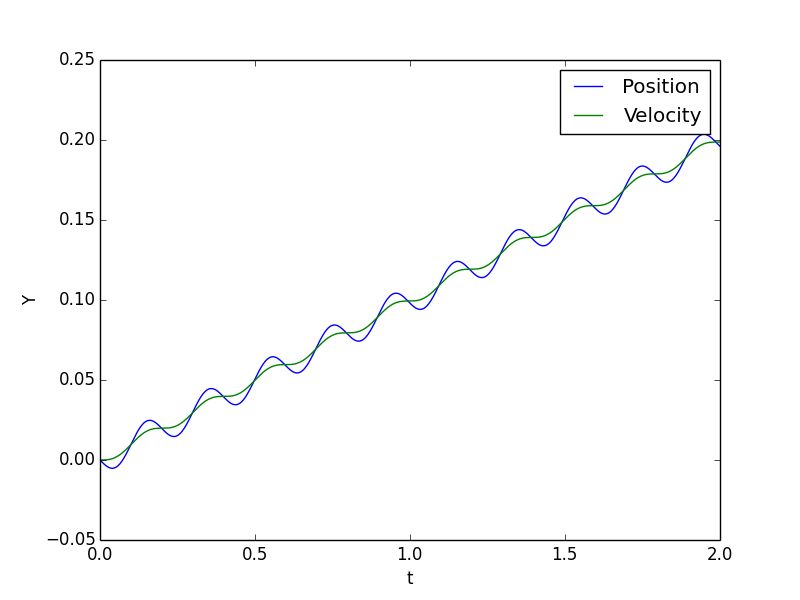
\includegraphics[scale=0.5]{oppg_r.png} 
        \caption{Graph}
\end{figure}

\pagebreak

%oppg s
\subsection{)}

\lstinputlisting{oppg_s.py}

\begin{figure}[h!]
        %\centering 
        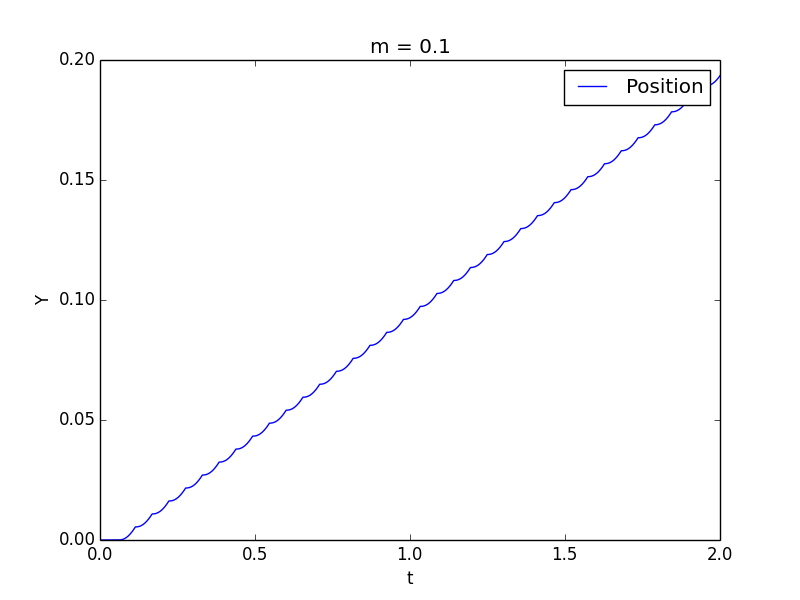
\includegraphics[scale=0.5]{oppg_s_1.png} 
        \caption{Graph}
\end{figure}
\begin{figure}[h!]
        %\centering 
        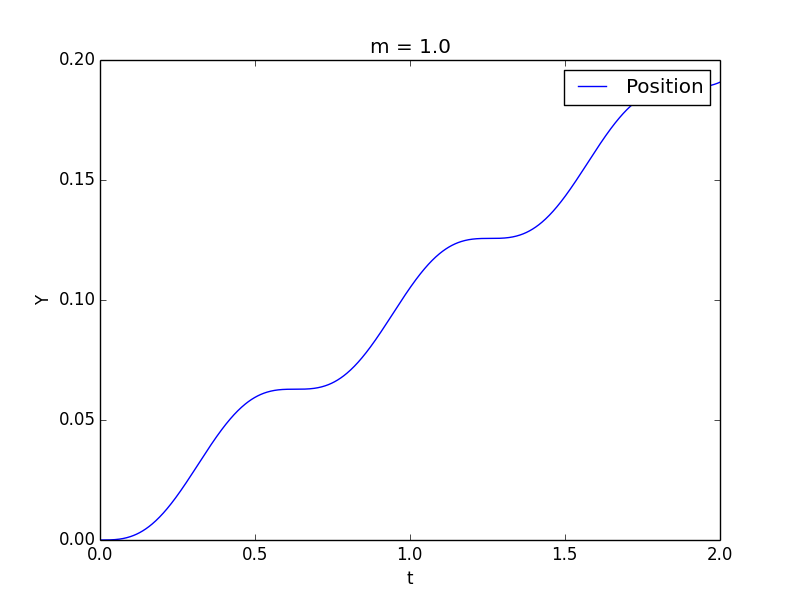
\includegraphics[scale=0.5]{oppg_s_2.png} 
        \caption{Graph}
\end{figure}

\pagebreak
%oppg t
\subsection{)}
This is m=0.1... I just forgot to change the title.
\begin{figure}[h!]
        \centering 
        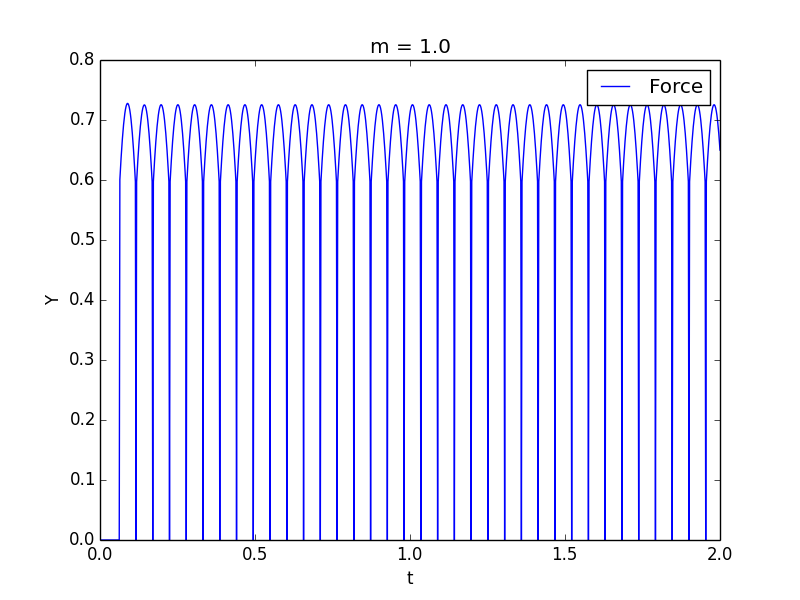
\includegraphics[scale=0.5]{oppg_t_1.png} 
        \caption{Graph}
\end{figure}

\begin{figure}[h!]
        \centering 
        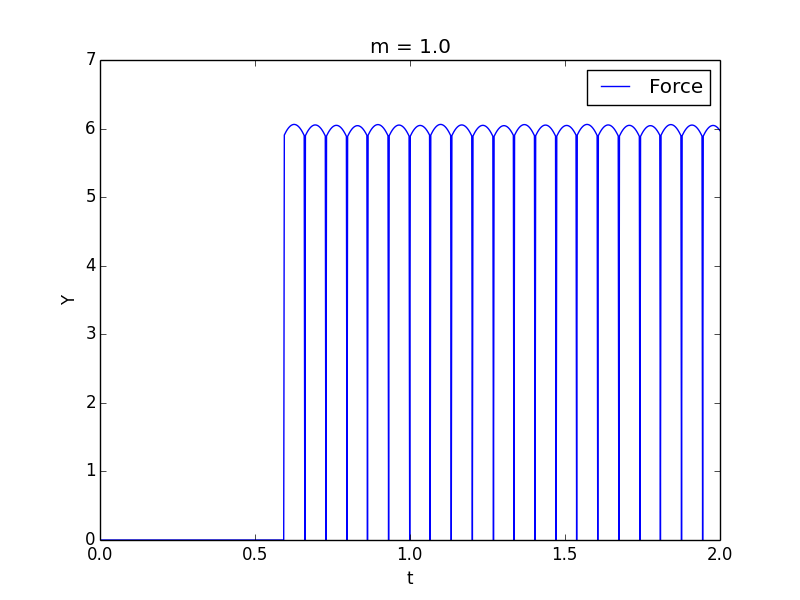
\includegraphics[scale=0.5]{oppg_t_2.png} 
        \caption{Graph}
\end{figure}

When $m = 1.0$, the gravitational force is bigger, so then the normal force is bigger, and further, the static friction si bigger.
Thats why the second graph starts later, because it needs more Force before it overcomes the static friction.


%oppg u
\subsection{)}
When k=10 and m = 0.1, we get the same graph and result as we did with m=1.0.

We can show why by setting up the net force in the x-direction:
\[\sum F_{\vec{i}} = F_{s} + F = 0\]
\[mg\mu_{s} = k\Delta L\]
So from this we can see that decreasing k by a factor of 10(dividing by 10), is the same as INcreasing m by a factor of 10(multiplying by 10).




\end{document}